% /**
% * Copyright 2012 Sergio García Mondaray
% *
% * This file is part of GodTIC-Templates (www.godtic.com).
% * 
% * GodTIC-Templates is free software: you can redistribute it and/or modify it
% * under the terms of the GNU General Public License as published by
% * the Free Software Foundation (version 3 of the License).
% * 
% * GodTIC-Templates is distributed in the hope that it will be useful, but
% * WITHOUT ANY WARRANTY; without even the implied warranty 
% * of MERCHANTABILITY or FITNESS FOR A PARTICULAR PURPOSE. 
% * See the GNU General Public License for more details.
% * 
% * You should have received a copy of the GNU General Public License 
% * along with GodTIC-Templates. If not, see http://www.gnu.org/licenses/.
% **/

%%%%%%%%%%%%%%%%%%%%%%%%%%%%%%%%%%%%%%%%%%%%%%%%%%%%%%%%%%%%%%%%%%%%%%
\documentclass[12pt]{beamer}% /**
% * Copyright 2012 Sergio García Mondaray
% *
% * This file is part of GodTIC-Templates (www.godtic.com).
% * 
% * GodTIC-Templates is free software: you can redistribute it and/or modify it
% * under the terms of the GNU General Public License as published by
% * the Free Software Foundation (version 3 of the License).
% * 
% * GodTIC-Templates is distributed in the hope that it will be useful, but
% * WITHOUT ANY WARRANTY; without even the implied warranty 
% * of MERCHANTABILITY or FITNESS FOR A PARTICULAR PURPOSE. 
% * See the GNU General Public License for more details.
% * 
% * You should have received a copy of the GNU General Public License 
% * along with GodTIC-Templates. If not, see http://www.gnu.org/licenses/.
% **/

\usepackage[utf8]{inputenc}
\usepackage[spanish]{babel}

\usetheme{/theme}
\usepackage{thumbpdf}
\usepackage{wasysym}
\usepackage{ucs}
\usepackage{pgf,pgfarrows,pgfnodes,pgfautomata,pgfheaps,pgfshade}
\usepackage{verbatim}
\usepackage{hyperref}
\usepackage{pifont}
\usepackage{color}
\usepackage{wrapfig}
\usepackage{graphicx}
\definecolor{mygreen}{rgb}{0,0.7,0.1}
\definecolor{myorange}{rgb}{1,0.5,0}

\graphicspath{{img/}} 
\DeclareGraphicsExtensions{.pdf,.png,.jpg}
\usepackage{listings}

\usepackage{color}
\definecolor{lightgray}{rgb}{.9,.9,.9}
\definecolor{darkgray}{rgb}{.4,.4,.4}
\definecolor{purple}{rgb}{0.65, 0.12, 0.82}

\lstdefinelanguage{JavaScript}{
  keywords={typeof, new, true, false, catch, function, return, null, catch, switch, var, if, in, while, do, else, case, break},
  keywordstyle=\color{blue}\bfseries,
  ndkeywords={class, export, boolean, throw, implements, import, this},
  ndkeywordstyle=\color{darkgray}\bfseries,
  identifierstyle=\color{black},
  sensitive=false,
  comment=[l]{//},
  morecomment=[s]{/*}{*/},
  commentstyle=\color{purple}\ttfamily,
  stringstyle=\color{red}\ttfamily,
  morestring=[b]',
  morestring=[b]"
}

\lstset{tabsize=4,
  showspaces=false,
  showtabs=false,
  frame=l,
  framerule=1pt,
  aboveskip=0.5cm,
  framextopmargin=3pt,
  framexbottommargin=3pt,
  framexleftmargin=18pt,
  framesep=.4pt,
  rulesep=.4pt,
  stringstyle=\ttfamily,
  showstringspaces = false,
  basicstyle=\footnotesize\ttfamily,
  keywordstyle=\bfseries,
  numbers=left,
  numbersep=6pt,
  numberstyle=\color[cmyk]{0.43, 0.35, 0.35,0.01}\bfseries\scriptsize\ttfamily,
  numberfirstline = true,
  breaklines=true,
  stepnumber=1,
  backgroundcolor=\color{white},
  xleftmargin=18pt,
  framexrightmargin=0pt,
  xrightmargin=0pt,
  language=JavaScript
}
 %%%%%% METADATOS %%
%%%%%%%%%%%%%%%%%%%%%%%%%%%%%%%%%%%%%%%%%%%%%%%%%%%%%%%%%%%%%%%%%%%%%%

\def\titulo{
  Atacando al Atacante
}
\def\autor{
  Jose Moruno Cadima\\
}
\def\email{
  moruno.jose@gmail.com\\

}
\date{Jornada de Seguridad Informática  - Septiembre  2014} % (Opcional) Puede tener varias líneas, estilos, etc

%%%%%%%%%%%%%%%%%%%%%%%%%%%%%%%%%%%%%%%%%%%%%%%%%%%%%%%%%%%%%%%%%%%%%%
\begin{document}% /**
% * Copyright 2012 Sergio García Mondaray
% *
% * This file is part of GodTIC-Templates (www.godtic.com).
% * 
% * GodTIC-Templates is free software: you can redistribute it and/or modify it
% * under the terms of the GNU General Public License as published by
% * the Free Software Foundation (version 3 of the License).
% * 
% * GodTIC-Templates is distributed in the hope that it will be useful, but
% * WITHOUT ANY WARRANTY; without even the implied warranty 
% * of MERCHANTABILITY or FITNESS FOR A PARTICULAR PURPOSE. 
% * See the GNU General Public License for more details.
% * 
% * You should have received a copy of the GNU General Public License 
% * along with GodTIC-Templates. If not, see http://www.gnu.org/licenses/.
% **/


\author{\autor}
\title{\titulo}

\frame{\titlepage}

\section*{}
\begin{frame}
  \frametitle{Índice}
  \framesubtitle{Contenido de la presentación}
  \tableofcontents[section=1,hidesubsections]
\end{frame}
\AtBeginSection[]
{
  \frame<handout:0>
  {
    \frametitle{Índice}
    \framesubtitle{Contenido de la presentación}

    \tableofcontents[currentsection,hideallsubsections]
  }
}
\AtBeginSubsection[]
{
  \frame<handout:0>
  {
    \frametitle{Índice}
    \framesubtitle{Contenido de la presentación}
    \tableofcontents[sectionstyle=show/hide,subsectionstyle=show/shaded/hide]
  }
}
\newcommand<>{\highlighton}[1]{
  \alt#2{\structure{#1}}{{#1}}
}
\newcommand{\icon}[1]{\pgfimage[height=1em]{#1}}

%% Título y subtítulo

\def\frametit{\insertsection}
\def\framesubtit{\insertsubsection}

%\newcommand{\slide}[1]{\begin{frame}\frametitle{\frametit}\framesubtitle{\framesubtit}#1\end{frame}}

\newenvironment{slide}[1][]
  {\begin{frame}[fragile,environment=slide,#1]
    \frametitle{\frametit}\framesubtitle{\framesubtit}}
  {\end{frame}}

\newenvironment{blankslide}[1][]
  {\begin{frame}[fragile,environment=blankslide,#1]
    \frametitle{}\framesubtitle{}}
  {\end{frame}}

%\newenvironment{slide}{\begin{frame}}{\end{frame}}
% \newenvironment{slidef}{\begin{xframe}}{\end{xframe}}
 %%%%%%%%% INICIO DEL DOCUMENTO %%
%%%%%%%%%%%%%%%%%%%%%%%%%%%%%%%%%%%%%%%%%%%%%%%%%%%%%%%%%%%%%%%%%%%%%%
\section{DISCLAIMER}

\begin{slide}

  \begin{alertblock}{Cuando se creo el Market}
     LOS ACTOS PRESENTES DERIVAN LA SITUACION FUTURA.

  \end{alertblock}

\end{slide}

\section{REGLAS Y NORMAS}

\begin{slide}


  \begin{itemize}
  \item Si hablo bajo.\pause
  \item Si hablo rapido. \pause
  \item Si hablo chino.\pause
  \item Si me equivoco.\pause
  \item Si no funciona algun demo.
  \end{itemize}
\end{slide}


\section{Whoami}

\begin{slide}
  
   \begin{center}
       Jose Moruno Cadima A.K.A Snifer.
   \end{center}
  
  \begin{itemize}
  \item Consultor Senior en Yanapti.\pause
  \item Desarrollador en Python, Perl, Ruby.\pause
  \item Analisis de Malware, Android Forensic, FirefoxOS \pause
  \item Integrante de Uremix, HackLab Cochabamba, Grampus Team.\pause
  \item Co-fundador de TkBreak y Sw-Craft
  \item Bloguero desenfrenado
  \item Mi pagina personal: http://www.sniferl4bs.com
  \end{itemize}
\end{slide}
%%%%%%%%%%%%%%%%%%
%%              %%
%% First Slide  %%
%%              %%
%%%%%%%%%%%%%%%%%%

\section{Que es el Hacking}
%%%%%%%%%%%%%%%%%%
%%              %%
%% Second Slide %%
%%              %%
%%%%%%%%%%%%%%%%%%

\subsection{Snifer anda loco como que zombies}

\begin{slide}
    \begin{figure}[h]
      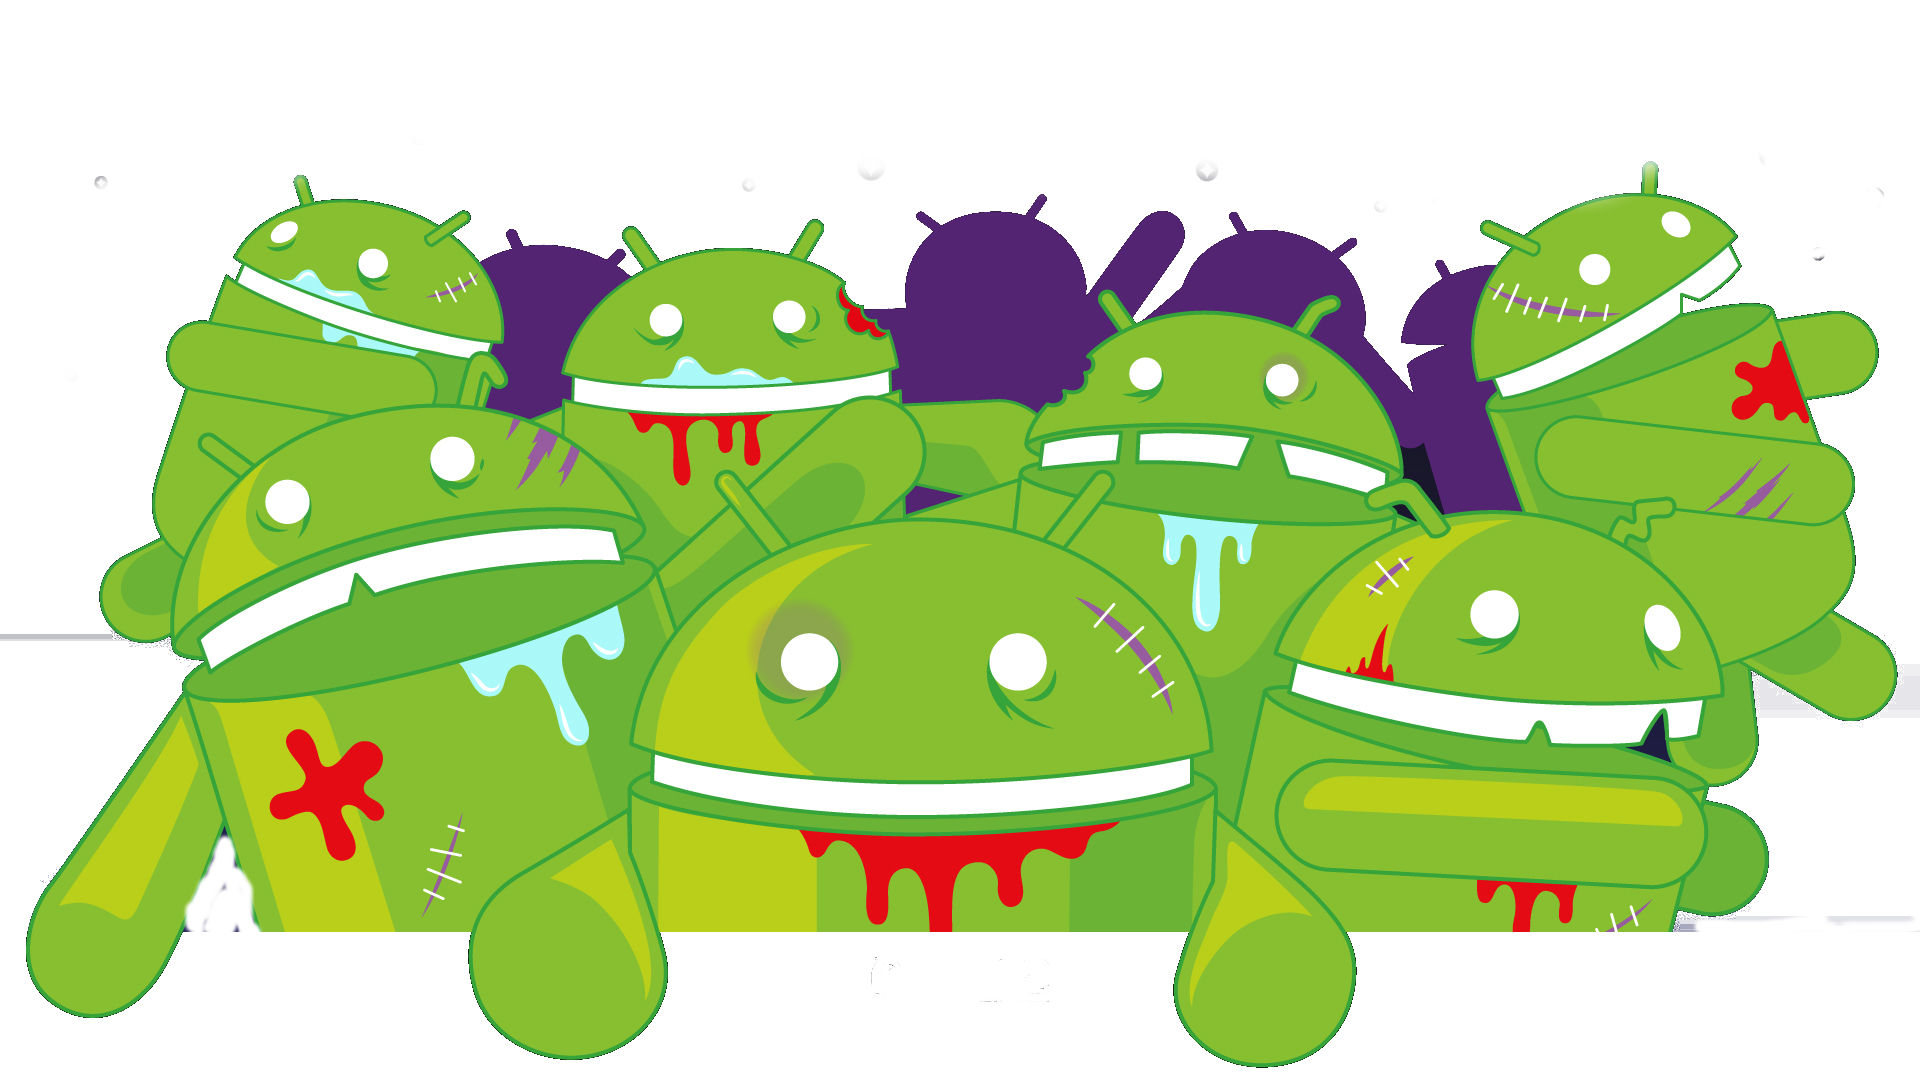
\includegraphics[height=0.7\textheight]{img/AndroZombie.png}
    \end{figure}
    Nuestro amigo es controlado...
\end{slide}
%%

%%
\subsection{Para quien va dirigida la charla}
\begin{slide}
 
  \begin{figure}[h]
      
\includegraphics[height=0.9\textheight]{img/camaleon.png}
  \end{figure}
\end{slide}

\begin{slide}
  \begin{figure}[h]
      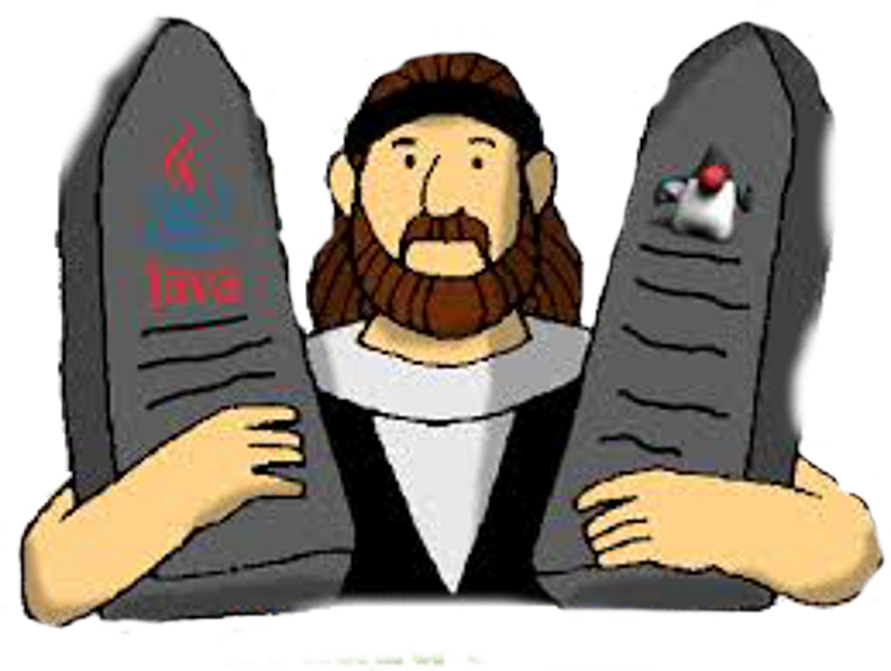
\includegraphics[height=0.9\textheight]{img/javas.png}
    \end{figure}
\end{slide}


\begin{slide}
  \begin{figure}[h]
      
\includegraphics[height=0.9\textheight]{img/zomdroid.png}
    \end{figure}
\end{slide}
%%      %%
%%%%%%%%%%
\subsection{Porque la charla}
\begin{slide}
 
  \begin{enumerate}
    \item Concientizar a un usuario normal.\pause
    \item No pidan permisos innecesarios.\pause
    \item Mostrar un poco de lo que me gusta.\pause
    \item Proteger nuestros datos personales.
  \end{enumerate}
\end{slide}
%%


\section{Historia}


\begin{slide}

  \begin{block}{Trabajo en Apple y Microsoft}
   Andy Rubin llevaba desde 1989 hasta 2003 trabajando como ingeniero en telecomunicaciones y en el mundo de los teléfonos móviles. Android Inc\pause
  \end{block}

  \begin{alertblock}{Cuando se creo el Market}
    Android 1.0 Apple Pie 22 de octubre de 2008.
  \end{alertblock}

\end{slide}

\begin{slide}

  \begin{exampleblock}{Andy es su nombre}
    El nombre del hombresito verde es Andy.
  \end{exampleblock}}

  \begin{exampleblock}{Andy Rubin}
    "La misma plataforma, el exacto sistema operativo que construimos para cámaras, eso se convirtió en Android para teléfonos inteligentes".
  \end{exampleblock}}

\end{slide}

%
\begin{slide}

  \begin{block}{Andy es su nombre}
   Es un software dañino cuyo objetivo es infiltrarse o dañar un equipo.
  \end{block}

  \begin{figure}[h]
      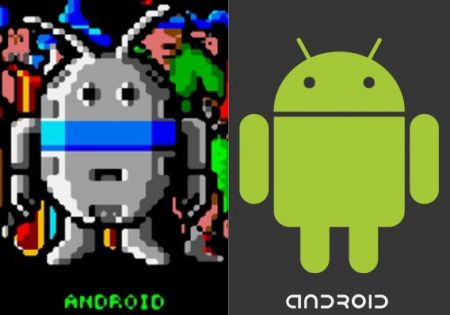
\includegraphics[height=0.6\textheight]{img/android-copia-videojuego.jpg}
    \end{figure}

\end{slide}
%%

\begin{slide}
  \begin{figure}[h]
      
\includegraphics[height=0.9\textheight]{img/gingerbread.png}
    \end{figure}
\end{slide}
%


\begin{slide}

     Los posibles Andy.
  \begin{figure}[h]
      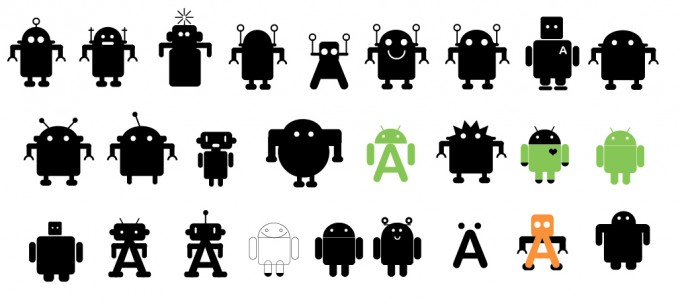
\includegraphics[height=0.5\textheight]{img/mutidroid.jpg}
    \end{figure}
\end{slide}

\begin{slide}

     Los posibles Andy.
  \begin{figure}[h]
      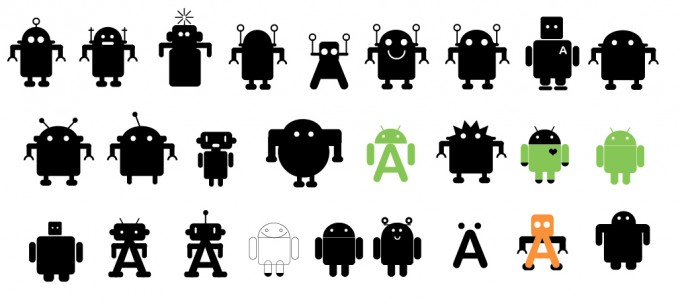
\includegraphics[height=0.5\textheight]{img/mutidroid.jpg}
    \end{figure}
\end{slide}

\section{La infeccion Zombie}
%%
\subsection{Permisos innecesarios en aplicaciones}
\begin{slide}
 Los culpables los desarroladores....
  \begin{enumerate}
    \item El mal manejo de permisos por parte de los desarrolladores.\pause
    \item No pidan permisos innecesarios.\pause
    \item Malas practicas de desarrollo.\pause
    \item Solicita todos los permisos asi te evitas de problemas.
  \end{enumerate}
\end{slide}
%%

\begin{slide}
  Una aplicacion solicita demasiados permisos para muestra unos botones.
    \begin{figure}[h]
      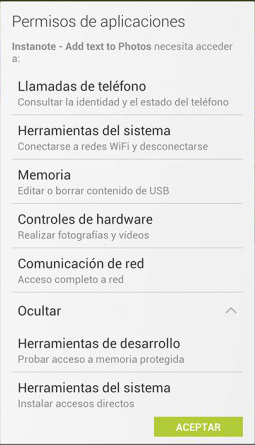
\includegraphics[height=0.9\textheight]{img/permisos.png}
    \end{figure}
\end{slide}

\begin{slide}
    \begin{figure}[h]
      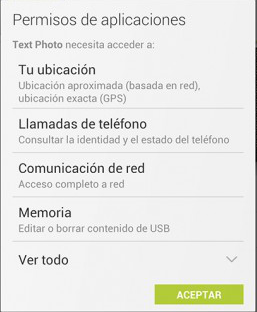
\includegraphics[height=0.9\textheight]{img/permisos1.png}
    \end{figure}
\end{slide}

\begin{slide}
    \begin{figure}[h]
      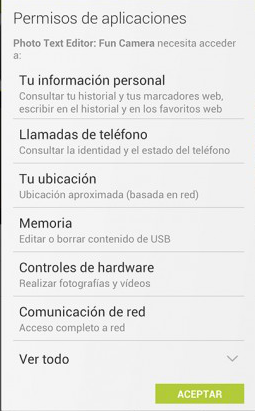
\includegraphics[height=0.9\textheight]{img/permisos2.png}
    \end{figure}
\end{slide}

\subsection{El Play Store el foco de infección}

\begin{slide}

 Play Store hasta 2012, no revisaba de forma alguna las aplicaciones que le enviaban los desarrolladores. \\
 El protocolo de actuación de Google se limitaba a revisar la aplicación (y retirarla, si se daba el caso)
 en base al número de denuncias recibidas por parte de los usuarios.
\end{slide}

\subsection{El mercado negro de las aplicaciones}

\begin{slide}

 ¿Quienes tienen aplicaciones de pago en el movil?\pause \\
 Legalmente compradas :) \pause \\
 ¿De donde consiguen esas aplicaciones?
  
\end{slide}


\begin{slide}
            Unofficial Android Marketplaces
    \begin{figure}[h]
      
\includegraphics[height=0.9\textheight]{img/MyCloud.jpeg}
    \end{figure}
\end{slide}

\subsection{Como sobrevivir al apocalipsis}

\begin{slide}
    \begin{figure}[h]
      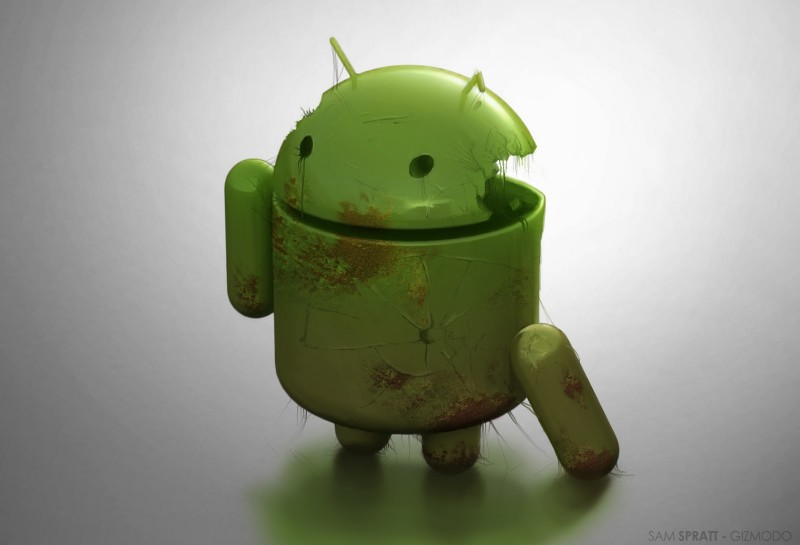
\includegraphics[height=0.9\textheight]{img/AndroidM.jpg}
    \end{figure}
\end{slide}

%%

\subsection{Lo que hacemos hoy... }


\begin{slide}
  \begin{exampleblock}{}
    LOS ACTOS PRESENTES DERIVAN LA SITUACION FUTURA.
  \end{exampleblock}}
\end{slide}


%%%%%%%%%%%%%%%%%%%%%%%%%%%%%%%%%%%%%%%%%%%%%%%%%%%%%%%%%%%%%%%%%%%%%%
%%%%%%%%%%%%%%%%%%%%%%%%%%%%%%%%% FIN %%%%%%%%%%%%%%%%%%%%%%%%%%%%%%%%
%%%%%%%%%%%%%%%%%%%%%%%%%%%%%%%%%%%%%%%%%%%%%%%%%%%%%%%%%%%%%%%%%%%%%%

\begin{blankslide}
  \begin{center}
    {\Large Gracias por su atención}
  \end{center}
   \begin{figure}[h]
      \begin{center}
        
\includegraphics[height=0.5\textheight]{img/sniferl4bs.png}
      \end{center}
    \end{figure}
  \begin{center}
    {\Large Twitter: @sniferl4bs}\\
    {\Large Skype:   sniferl4bs}
  \end{center}
  \begin{flushright}
    {\bf \autor}\\
    {\tt \email}\\[0.2cm]
    %% Por favor, respeta esta referencia al autor de la plantilla
    {\scriptsize Presentación compuesta con \LaTeX\ }
  \end{flushright}
\end{blankslide}

\end{document}
